\chapter{فونت و نویسه‌ها}\label{chp:chap2}
\thispagestyle{empty}
% \rhead{\leftmark}
\normalfootnotes
\section{انواع فونت‌ها در رایانه}
به یاد خالق فونت «وزیرمتن» و «فونت ساحل»  مرحوم صابر راستی کردار که فارسی نوشتن را برای فارسی نویسان عصر تکنولوژی زیبا کرد.
در حالت کلی تمامی فونت هایی که شما با آن سروکار دارید، در سه دسته کلی طبقه‌بندی می‌گردد.
\begin{description}
 \item[ فونت‌های \lr{bitmap}:] فونت‌های \lr{Bitmap} به صورت ماتریسی از نقاط بیان می‌شوند. به همین علت این فونت‌ها به سخت افزار سیستم وابسته‌ هستند و فقط در یک \lr{resolution} معین به کار می‌آیند. یک \lr{bitmap} روی صفحه ۷۵\lr{DPI} با وجود یک چاپگر ۱۲۰۰\lr{DPI} همچنان به صورت ۷۵\lr{DPI} خواهد بود. فونت‌های \lr{bitmap} صفحه نمایش معمولاً دارای پسوند \lr{bdf} یا \lr{pcf} می‌باشند. این فونت‌ها اغلب در پنجره‌ها، کنسول‌ها و ویرایشگرهای متنی کاربرد دارند، زیرا در این محلها عدم مقیاس پذیری مسئله چندان مهمی نیست.
 \item[فونت‌های \lr{Outline}:] به این دسته از فونت‌ها اصطلاحا فونت‌های برداری (\lr{vector font}) نیز گفته می‌شود. در این دسته از فونت‌ها، توصیف کلی فونت به صورت یکسری قواعد برداری و روابط ریاضیاتی بیان می‌شود، بدین‌سان این فونت‌‌ها تا هر اندازه دلخواهی توانایی مقیاس‌پذیر بودن دارند. برخی از انواع فونت های این دسته به شرح زیر است.
 \begin{latin}
\begin{itemize}
 \item Post script Type 1
    \item Post script Type 3
     \item True Type
     \item Open Type
\end{itemize}
\end{latin}
\item[فونت‌ها نوع\lr{Stroke}:] این دسته از فونت ها از یکسری خطوط به همراه توصیفی از نحوه چیدمان خطوط در کنار یکدیگر، تشکیل شده است. فونت های \lr{metafont }در این دسته جای می‌گیرند
\end{description}
\section{فونت در \lr{xepersian}}
در \lr{xepersian} شما می توانید سه دسته فونت کلی تعریف کنید. این سه دسته عبارت اند از:
\begin{itemize}
\item 
فونت مخصوص عبارات فارسی که با دستور \lr{settextfont} تعیین می شود، به عنوان مثال:
\begin{latin}
\begin{lstlisting}[style=Tex]
\settextfont{Vazirmatn}
\end{lstlisting}
\end{latin}
    فونت برای عبارات انگلیسی. اولا دقت کنید که برای این که \lr{xepersian} بتواند بفهمد که کلمه شما انگلیسی است، بدین‌سان شما باید کلمه و یا عبارت خود را درون دستور
 \lr{\textbackslash{lr}\{\}} قرار دهید، مثلا:
\begin{latin}
\begin{lstlisting}[style=Tex]
 \lr{English Words}
\end{lstlisting}
\end{latin}
و توسط دستور \lr{setlatintextfont} نیز یک فونت انگلیسی تعریف کنید. مانند آن چه که در ادامه آمده است.
\begin{latin}
\begin{lstlisting}[style=Tex]
\setlatintextfont{Vazirmatn}
\end{lstlisting}
\end{latin}
\item 
    در ضمن شما می توانید یک فونت هم برای اعداد و ارقام در فرمول های ریاضی تعریف کنید. به صورت زیر:
\begin{latin}
\begin{lstlisting}[style=Tex]
\setdigitfont{Vazirmatn}
\end{lstlisting}
\end{latin}
دقت کنید که به صورت پیش فرض اعداد و ارقام به صورت فارسی در فرمول ها در لاتک نوشته می شود، اگر بخواهد اعداد و ارقام به صورت انگلیسی در فرمول ها ظاهر شوند، کافی است دستور زیر را بنویسید:
\begin{latin}
\begin{lstlisting}[style=Tex]
\DefaultMathsDigits
\end{lstlisting}
\end{latin}
\end{itemize}
در مورد نحوه تنظیم اندازه فونت در بخش بعدی سخن به میان خواهد آمد. 
\section{اندازه فونت}
قبل از این‌که وارد بحث اصلی شویم، ابتدا باید بفهمیم که منظور از اندازه فونت چیست؟ در یک تعریف کلی به تفاوت ارتفاع بین بلندترین حرف و کوتاهترین حرف، اندازه فونت گویند.
\begin{figure}[h!]
 \centering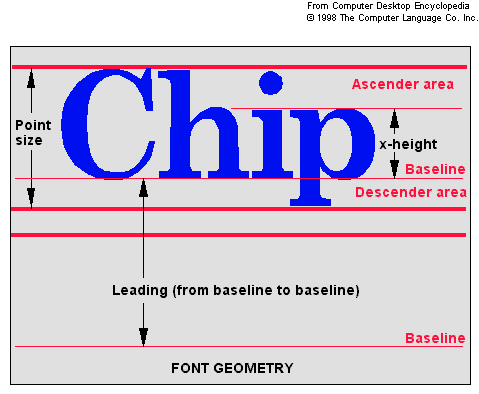
\includegraphics[scale=0.4]{8E8XO.jpg}
  \caption{تعریف اندازه فونت برای فونت های انگلیسی}
\end{figure}
اگر تاکنون با \lr{word} کار کرده اید، حتما فونت ها را با معیاری به نام اندازه می شناسید. این معیار اندازه با معیار اندازه بر حسب \lr{point} در \lr{Latex} متفاوت است. البته این تفاوت برای همه فونت ها یکسان نیست، لذا کار کمی پیچیده می شود. اما اگر در ادامه نیز همراهی کنید، فکر کنم به خوبی می توانید موضوع را متوجه شوید. فرض کنید که می‌خواهید نوشتار خود را با اندازه فونت ۱۴ در \lr{Latex} تایپ کنید. برای این کار باید چند نکته و گام را در نظر بگیرید.
\begin{figure}[h!]
 \centering
\includegraphics[scale=0.4]{FontSizePersian.jpg}
 \caption{تعریف اندازه فونت برای فونت های انگلیسی}
\end{figure}
\subsubsection{گام نخست}
در ابتدا باید یک فونت پایه برای نوشتار خود انتخاب کنید. در کل سه اندازه استاندارد برای نوشتار‌های رسمی وجود دارد:
\begin{itemize}
 \item     اندازه 10\lr{pt} که اندازه کوچک نامیده شده (که فونت‌اندازه پیشفرض تک می‌باشد.)
  \item     اندازه 11\lr{pt} که اندازه متوسط نامیده می‌شود.
   \item    اندازه 12\lr{pt} که اندازه بزرگ محصوب می‌شود.
برای تنظیم اندازه فونت پایه در lr{Latex}\ چندین روش وجود دارد، که ما در ادامه به دو مورد از آن‌ها اشاره می‌کنیم.
     \item   می توانید این مورد را در قسمت اختیاری \lr{documentclass} بنویسید. مانند:

\begin{latin}
\begin{lstlisting}[style=Tex]
\documentclass[12pt]{report}
\end{lstlisting}
\end{latin}
با این کار شما اندازه فونت پایه را 12\lr{pt} گذاشتید.

     \item   اگر دارید فایل استایل می نویسید، در دستور \lr{loadClass} عدد 12\lr{pt} را بگذارید.
\begin{latin}
\begin{lstlisting}[style=Tex]
 \LoadClass[12pt]{.....}
\end{lstlisting}
\end{latin}
     \item   در اکثر استایل‌های پیش‌فرض \lr{Latex} به مانند \lr{report، book، article، letter} و ... اندازه پیش‌فرض 10\lr{pt} است
\end{itemize}
\subsubsection{گام دوم}
اکنون شما می‌توانید با دو روش اندازه فونت خود را تعیین کنید. در روش اول، از دستور Scale در تعریف فونت استفاده می‌گردد. به عنوان مثال:
\begin{latin}
\begin{lstlisting}[style=Tex]
\settextfont[Scale=1.4]{XB Niloofar}
\setlatintextfont[Scale=1.3]{Times New Roman}
\end{lstlisting}
\end{latin}
برای مثال با اندازه فونت پایه 10\lr{pt} و Scale=1.2 اندازه فونت برابر با 12\lr{pt} خواهد شد، و یا برای اندازه فونت پایه 12\lr{pt} و \lr{Scale=1.2} اندازه فونت برابر با 14.4 خواهد شد. روش دوم مسستقل از اندازه فونت پایه است، در این روش در هرجایی از متن که می‌خواهید از دستور \lr{fontsize} به صورت زیر استفاده کنید.
\begin{latin}
\begin{lstlisting}[style=Tex]
\fontsize{x}{y}\selectfont
\end{lstlisting}
\end{latin}
در این روش از هر جایی از متن که دستورات فوق زده شود، اندازه فونت به مقدار x تنظیم خواهد شد و اندازه فاصله خط کرسی به y. البته هر جایی از متن که خواستید می‌توانید این اندازه را تغییر دهید به عنوان مثال، کد زیر را در نظر بگیرید.
\begin{latin}
\begin{lstlisting}[style=Tex]
\documentclass[10pt]{article}
\usepackage{xepersian}
\settextfont{XB Niloofar}
 
\begin{document}
%*\rl{در حالتی که اندازه‌ای تعریف نشده، نوشتار با اندازه فونت پایه چاپ می‌شود.}*)
\fontsize{13}{14}\selectfont
%*\rl{از این قسمت به بعد اندازه فونت ۱۳ خواهد شد.}*)
\fontsize{16}{17}\selectfont
%*\rl{از این قسمت به بعد اندازه فونت 16 خواهد شد.}*)
\end{document}
\end{lstlisting}
\end{latin}
خروجی در شکل زیر نشان داده شده است. 
\begin{figure}[h!]
 \centering
\includegraphics[scale=0.5]{Fontsizelatex.png}
 \caption{مثالی از تغییر اندازه فونت با دستور \lr{fontsize}}
 \end{figure}
 در کل بهتر است از روش \lr{fontsize} برای تغییر اندازه فونت به جای روش \lr{Scale} استفاده کنید. دلیلش هم این است که (۱) کیفیت در مقیاس‌های بزرگ پایین می‌آید زیرا که شما تنها ابعاد را بزرگ یا کوچک می‌کنید (۲) هیچ کنترلی روی فاصله خط کرسی وجود ندارد
\subsubsection{گام سوم}
البته قضیه بدین‌جا ختم نمی‌شود. برطبق این پست این موضوع در فونت‌های فارسی ظاهرا رعایت نمی‌شود. حروف فارسی به گونه‌ای هستند که این ارتفاع در آنها از حروف انگلیسی بیشتر است. بنابراین چنانچه ی متن فارسی با فونت ۱۲ داشته باشیم و در همان متن از فونت ۱۲ انگلیسی هم استفاده کنیم، حروف فارسی کمی کوچکتر به نظر می‌رسند. به همین دلیل در برخی از فونتها به طور عمد سایز فونت‌های فارسی را الکی بزرگ کردند تا از لحاظ ظاهری شل آنها با فونتهای انگلیسی همخوان باشد. این کار باعث به هم ریختن استاندارد شده است. در همان پست یاد شده کدهایی قرار داده شده است که شما می‌توانید نسبت دقیق را بدست آورید.
\section{فونت فارسی و انگلیسی}
در نرم افزار \lr{word} وقتی شما از یک فونت به عنوان نمونه \lr{B Nazanin} استفاده می کنید، \lr{word} در هنگام مواجه با کلمات انگلیسی، این کلمات را به یک فونت پیش فرض تبدیل می کند. چرا که اغلب فونت هایی که ما با آن ها کار می کنیم، تنها می توانند زبان فارسی و یا انگلیسی را پشتیبانی کنند. مثلا \lr{B Nazanin} فقط برای پشتیبانی از زبان فارسی است و نه برای انگلیسی. اما در \lr{LATEX} این گونه نیست. برای حل این مشکل دو راه حل دارید:
\begin{enumerate}
 \item     از فونت‌هایی استفاده کنید که هم فارسی را پشتیبانی می کنند و هم انگلیسی را، به مانند فونت‌های سری \lr{XB} مثل \lr{XB Niloofar}. برای دانلود فونت‌های از این قبیل به پیوند \lr{X Series fonts} مراجعه کنید.
  \item     در این روش، می بایست عبارات انگلیسی در متن فارسی را در داخل یک \textbackslash{lr}\{\} قرار دهید تا فهمیده شود که این عبارت باید با فونت انگلیسی نوشته شود. در این روش عبارت‌های انگلیسی با فونت انگلیسی در متن ظاهر می‌گردد.
\end{enumerate}
% نکات:
\begin{itemize}
 \item     در کل به نظر من راه حل دوم بهتر است.
  \item  در روش اوّل، نیازی نیست که کلمات انگلیسی خود را درون دستور \textbackslash{lr}\{\} قرار دهید.
\end{itemize}
\section{نحوه تعریف فونت های دیگر}
توسط دستورات 
\lr{defpersianfont} و \lr{deflatinfont} به ترتیب می توان یکسری فونت فارسی و انگلیسی دیگر تعریف کرد که در جاهای دیگر متن بتوان از آن استفاده کرد. مثلا در ادامه ما دو فونت تعریف کرده ایم:
\begin{latin}
\begin{lstlisting}[style=Tex]
\defpersianfont\myFafont[Scale=.8]{XM Traffic}
\deflatinfont\myEnfont[Scale=.9]{Adobe Arabic}
\end{lstlisting}
\end{latin}
هرگاه خواستیم یک عبارت از متن ما به صورت فونت های یادشده نوشته شود کافی است به صورت زیر عمل کنیم:
\begin{latin}
\begin{lstlisting}[style=Tex]
\myFafont{.................}
\end{lstlisting}
\end{latin}
که به جای نقطه چین کافی است عبارتی را که می خواهیم به صورت آن فونت در آید را قرار دهیم. 
\section{فونت‌های مورد نیاز قالب \lr{iut-thesis}}
تمامی فونت‌های مورد نیاز این قالب در پوشه \lr{fonts} قرارد دارد که باید آنها را نصب کنید. نصب فونت در لینوکس با قرار دادن پوشه‌ای حاوی فونت‌ها با نام \lr{.fonts} در پوشه خانگی و یک بار لاگین مجدد انجام می‌شود. در ویندوز نیز از طریق کنترل پانل و بخش فونت با کپی کردن فونت‌ها این کار صورت می پذیرد.
